\chapter{Оценка качества сварного соединения по сигналам спектрометрической системы}

\section{Постановка задачи}

В данной части работы исследованы спектральные сигналы, зарегистрированные в процессе лазерной сварки образцов из стали 09Г2С толщиной 3~мм. Сварка выполнялась с использованием волоконного лазера MAXPhotonics MFSC-3000, роботизированной системы перемещения FANUC M710iC/70 и оптической схемы WSX ND40. Длина волны лазерного излучения --- 1080~нм, диаметр оптического волокна --- 100~мкм, фокусное расстояние коллиматора --- 100~мм, фокусное расстояние фокусирующей оптики --- 250~мм. Диаметр пятна в фокусе составлял 0,14~мм. В качестве защитного газа использовался аргон с расходом 15~л/мин. Рассматривалось стыковое соединение.

В отличие от коаксиальной фотодиодной системы, рассмотренной в предыдущей главе, спектрометрическая система регистрировала не временную зависимость интегральной интенсивности, а распределение интенсивности излучения по длинам волн. При этом спектрометр был закреплён статично относительно сварочного стола. Следовательно, система наблюдала фиксированную область пространства, тогда как лазерный пучок перемещался вдоль образца. Эта особенность принципиальна для дальнейшей интерпретации результатов, поскольку отдельный спектр не может быть напрямую сопоставлен с произвольной точкой сварного шва без дополнительной локальной разметки.

Целью анализа являлась проверка возможности оценки качества сварного соединения по спектральным признакам. Как и в предыдущей главе, основное внимание уделялось непровару. Для каждого образца была известна величина \(h_i\), определённая по результатам макроанализа. Значение \(h_i = 0\) соответствует полному проплавлению, а \(h_i > 0\) --- наличию непровара. В данной главе рассматривается прежде всего качественная постановка задачи, то есть определение наличия или отсутствия непровара по спектральным данным.

\section{Структура экспериментальных данных}

Исходные спектральные данные были представлены в виде файлов формата Raw8. Каждый файл содержал служебный заголовок, после которого располагались массивы длин волн и соответствующих им интенсивностей. После чтения данных каждый спектр представлялся как зависимость
\[
I = I(\lambda),
\]
где \(\lambda\) --- длина волны, а \(I\) --- зарегистрированная интенсивность оптического излучения.

В исходных данных присутствовали три спектрометрических канала. Для дальнейшего анализа был выбран основной канал \texttt{1712307U3}, поскольку в нём наблюдался наиболее выраженный спектральный максимум. Диапазон длин волн для данного канала составлял от \(467,396\) до \(708,946\)~нм. Остальные спектрометрические каналы в данной части работы не рассматривались.

Результаты контроля качества были заданы в отдельной таблице макроанализа. Сопоставление спектров с результатами контроля выполнялось по идентификатору образца. Всего для выбранного канала было найдено 3131 спектральных записей, которые удалось сопоставить с образцами, имеющими известное значение \(h_i\). Спектральные данные были доступны для 32 образцов.

Для каждого образца значение \(h_i\) определялось как максимальное значение по макрошлифам. Такой подход был выбран потому, что при контроле качества сварного соединения изделие оценивается по наиболее неблагоприятному локальному участку. Если непровар присутствует хотя бы на одном сечении, усреднение по нескольким макрошлифам может искусственно уменьшить выраженность дефекта. Использование максимального значения \(h_i\) поэтому лучше соответствует практической логике браковки.

\section{Предварительный отбор спектров}

Особенностью исходного набора являлось наличие спектральных записей с выраженным полезным сигналом и записей, близких к шумовому уровню. Такие слабые сигналы не отражали устойчивую спектральную картину излучения зоны сварки и могли ухудшать дальнейшее извлечение признаков. Поэтому перед расчётом признаков был выполнен предварительный отбор спектров.

Фильтрация выполнялась отдельно внутри каждого образца. Это важно, поскольку абсолютный уровень сигнала может различаться между экспериментами, и единый глобальный порог по интенсивности мог бы привести к смещённому отбору. Для каждого спектра рассчитывались средняя интенсивность, суммарная интенсивность и отношение максимума к среднему уровню. Последний параметр использовался как простая характеристика выраженности спектрального максимума:
\[
r_{\max} = \frac{I_{\max}}{\overline{I}}.
\]
Спектр сохранялся для дальнейшего анализа только в том случае, если он проходил отбор по уровню интенсивности, интегральному сигналу и выраженности максимума.

После предварительной фильтрации из 3131 спектральных записей осталось 356 спектров. Таким образом, дальнейший анализ выполнялся не по всем исходным Raw8-файлам, а по тем спектрам, которые содержали достаточно выраженный оптический сигнал.

\section{Предобработка спектральных сигналов}

Для повышения устойчивости признакового описания были рассмотрены несколько представлений спектрального сигнала. Помимо исходного спектра использовались сглаженный спектр, спектр после удаления базовой линии, а также сглаженный спектр после удаления базовой линии. Такая схема позволяет отдельно учитывать общий вид спектра, влияние высокочастотных флуктуаций и вклад медленно изменяющегося фонового уровня.

На рис.~\ref{fig:spectrum_processing_example} приведён пример предварительной обработки спектрального сигнала. Видно, что сглаживание уменьшает локальные флуктуации интенсивности, а удаление базовой линии позволяет более явно выделить форму спектрального распределения относительно фоновой составляющей.

\begin{figure}[H]
    \centering
    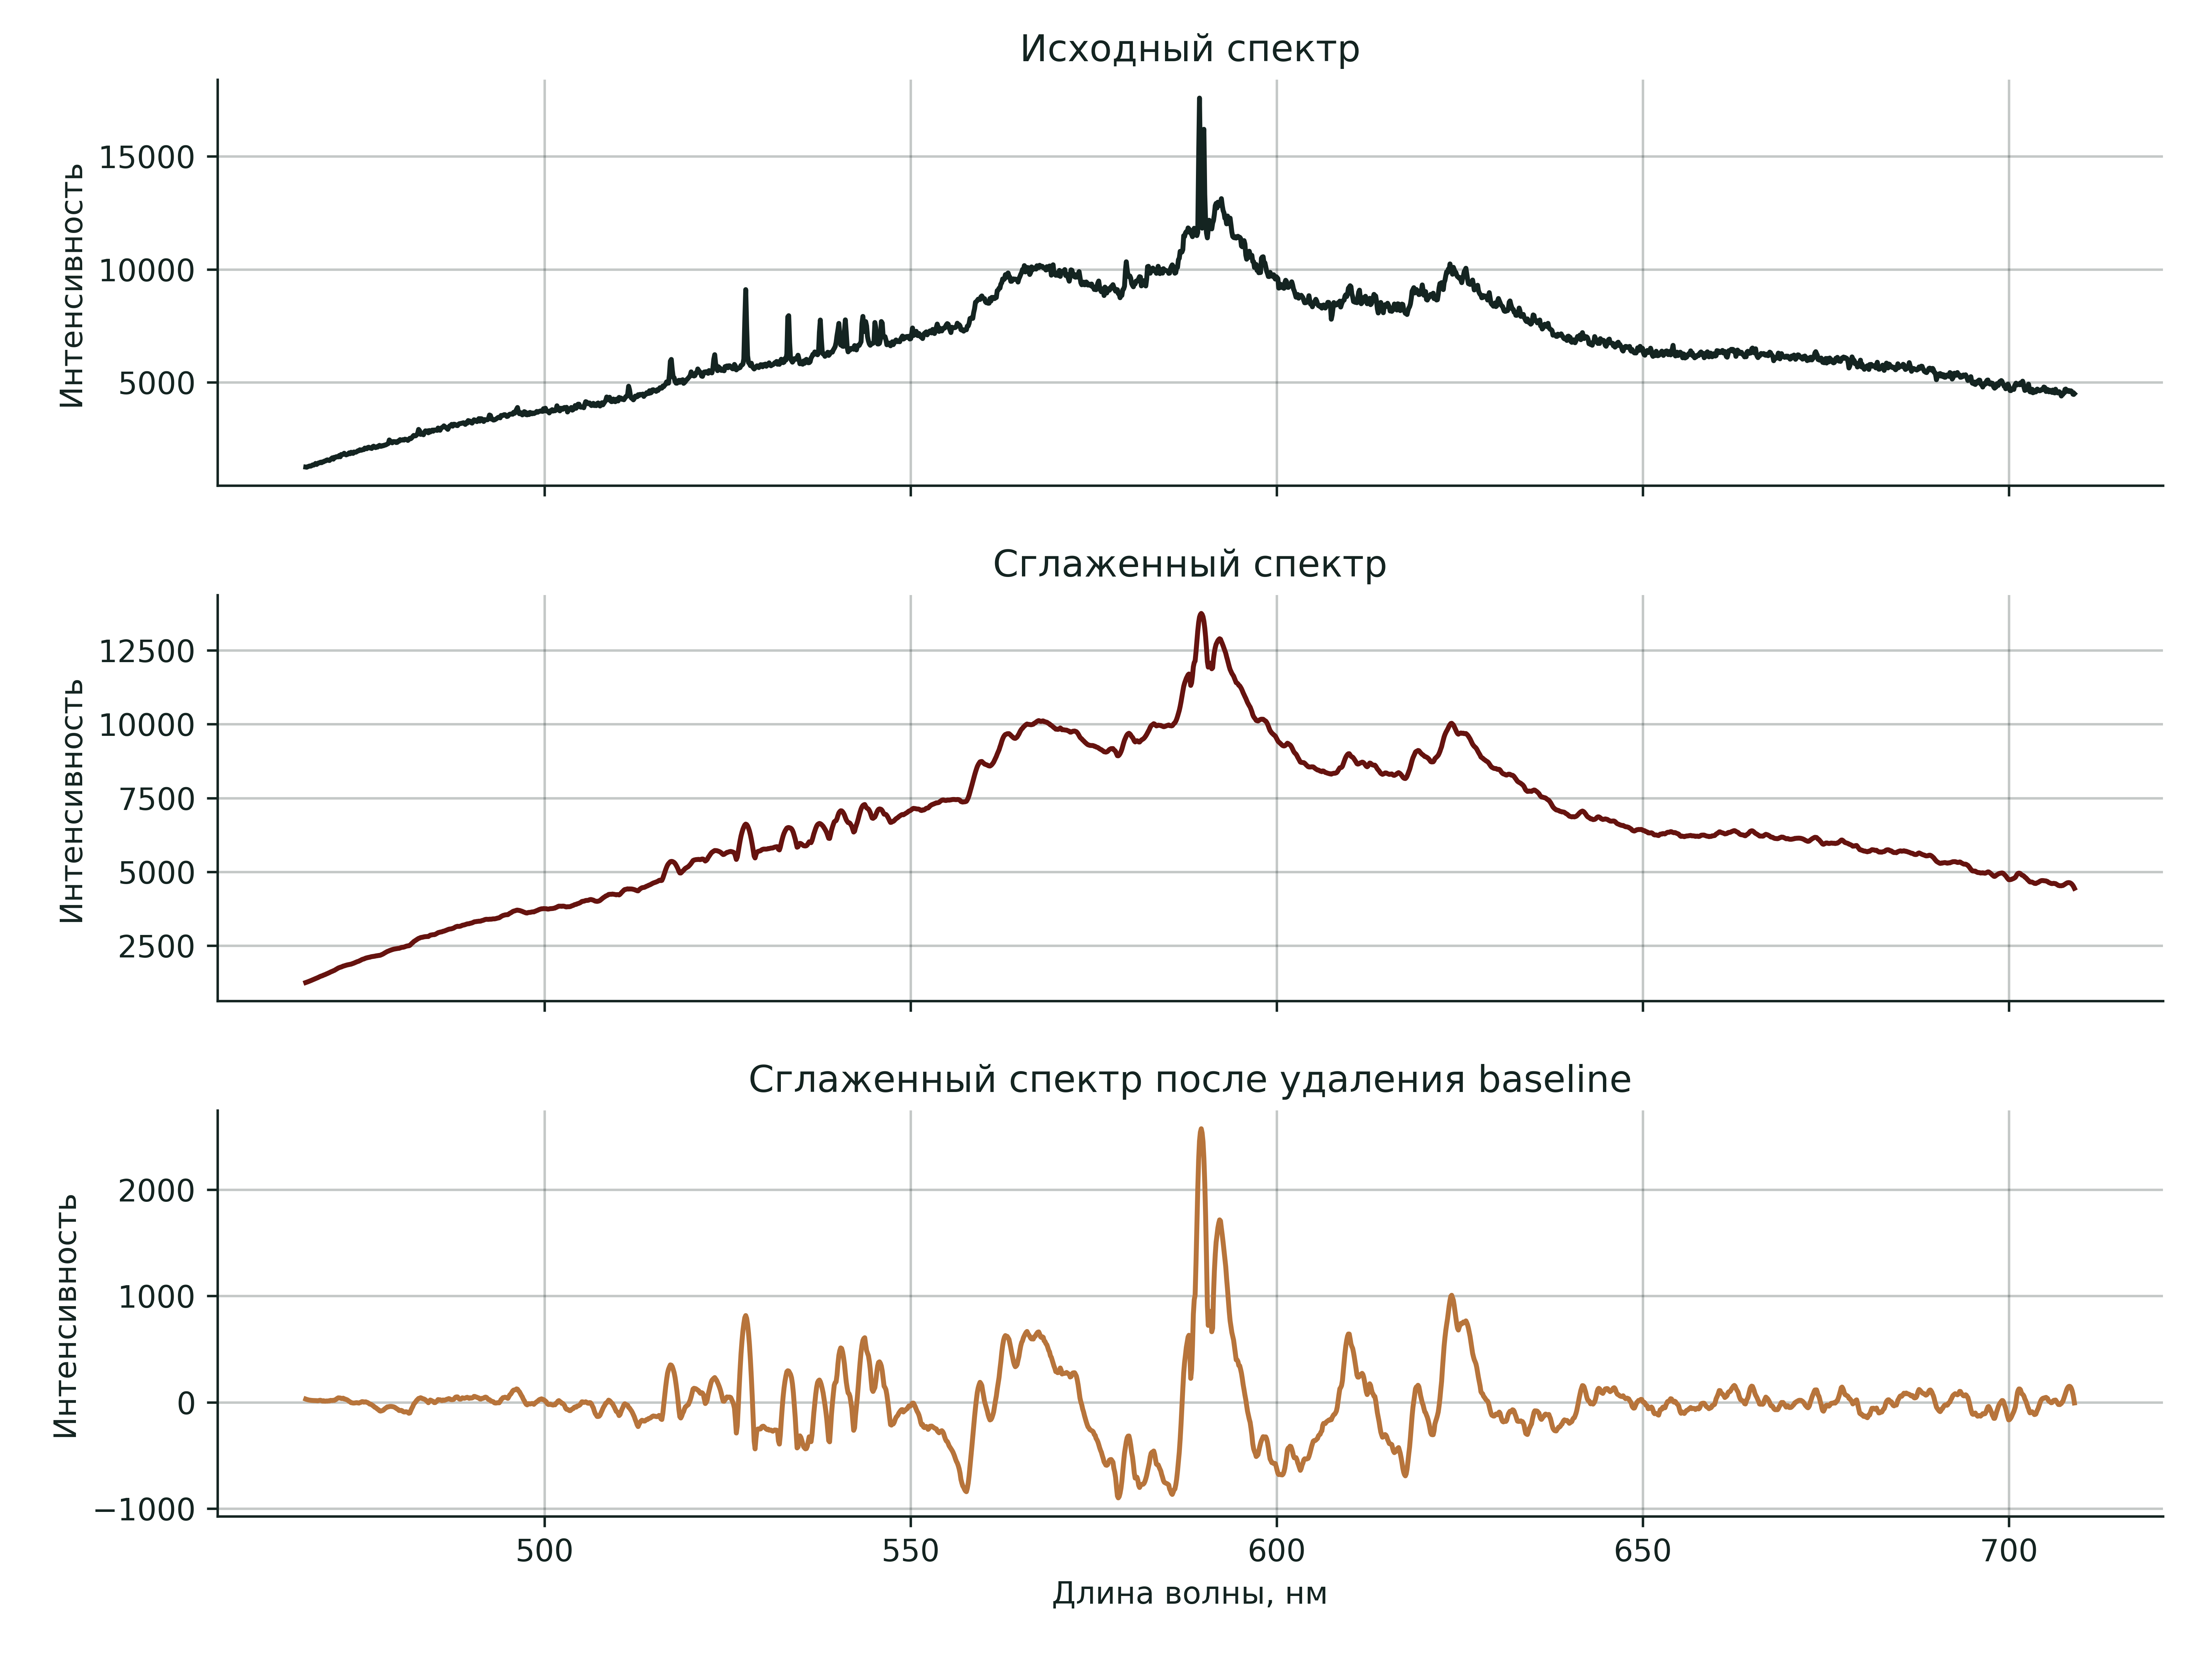
\includegraphics[width=0.9\textwidth]{figures/spectrum_processing_example.png}
    \caption{Пример предварительной обработки спектрального сигнала}
    \label{fig:spectrum_processing_example}
\end{figure}

Следует отметить, что предварительная обработка в данном случае не рассматривалась как самостоятельный способ классификации. Она использовалась для формирования нескольких вариантов признакового описания одного и того же спектра. Это позволяло проверить, какие характеристики оказываются более полезными: рассчитанные по исходному сигналу или по сигналу после сглаживания и коррекции базовой линии.

\section{Расчёт спектральных признаков}

В отличие от временных сигналов фотодиодной системы, спектральные данные не требуют оконного представления. Каждый спектр уже является конечным описанием распределения интенсивности излучения по длинам волн. Поэтому в данной части работы признаки рассчитывались по всему спектру целиком.

Прямое использование полного массива интенсивностей не является удобным для рассматриваемой задачи. С одной стороны, спектр содержит большое количество точек. С другой стороны, число независимых образцов невелико. Поэтому исходная зависимость \(I(\lambda)\) была преобразована в набор признаков, описывающих уровень, форму и частотную структуру спектра.

Первая группа признаков включала статистические характеристики интенсивности: среднее значение, стандартное отклонение, минимум, максимум, размах, среднеквадратичное значение, энергию, асимметрию, эксцесс, энтропию и квантили. Эти признаки характеризуют общий уровень излучения и распределение интенсивности по спектру.

Вторая группа была связана с пиковыми характеристиками. Для спектра определялись положение основного максимума, его интенсивность и признаки, связанные с выраженностью пика. Такие параметры важны, поскольку в выбранном спектрометрическом канале полезный сигнал проявлялся не только изменением общего уровня, но и наличием выраженного максимума в спектральном распределении.

Третью группу составляли диапазонные признаки. Для заданных диапазонов длин волн рассчитывались интегральные и относительные интенсивности. В отличие от простого максимума, такие признаки описывают распределение энергии по участкам спектра и позволяют учитывать не только локальный пик, но и изменение формы спектральной кривой в целом.

Дополнительно рассчитывались признаки на основе преобразования Фурье зависимости \(I(\lambda)\). В этом случае преобразование выполнялось не по времени, а по оси длин волн, поэтому соответствующие частоты имеют размерность \(\text{нм}^{-1}\). Эти признаки не следует интерпретировать как временные частоты колебаний процесса. Они характеризуют структуру изменения интенсивности вдоль спектральной оси. По амплитудному спектру рассчитывались доминирующая частота, полная энергия, а также доли энергии в низкочастотной, среднечастотной и высокочастотной областях.

\section{Агрегация признаков на уровне образца}

На первом этапе каждый отобранный спектр рассматривался как отдельная запись, для которой вычислялся набор признаков. Однако целевой параметр \(h_i\) был определён не для отдельного спектра, а для образца в целом по результатам макроанализа. Это создаёт важное методическое ограничение: отдельный спектр не имеет собственной локальной метки качества.

Кроме того, спектрометрическая система была закреплена статично относительно стола. Вследствие этого последовательность спектров отражает прохождение зоны сварки через область наблюдения, но не даёт прямого соответствия между конкретным спектром и конкретным макрошлифом. Поэтому основная постановка анализа была сформулирована на уровне образца.

Для этого признаки сначала рассчитывались для отдельных спектров, а затем агрегировались по идентификатору образца. Для каждого признака внутри одного образца вычислялись среднее значение, стандартное отклонение, минимум и максимум. Также учитывалось число спектров, оставшихся после предварительного отбора. После такой агрегации объектом классификации становился один образец, а не отдельная спектральная запись.

Всего в основной классификационной постановке рассматривались 32 образца. Из них 23 соответствовали полному проплавлению, а 9 --- непровару. Такое распределение классов является несбалансированным, что необходимо учитывать при интерпретации качества моделей.

\section{Качественная оценка непровара по спектральным признакам}

Качественная постановка задачи состояла в определении наличия непровара по агрегированным спектральным признакам. Бинарная метка качества задавалась по величине \(h_i\):
\[
y =
\begin{cases}
0, & h_i = 0,\\
1, & h_i > 0.
\end{cases}
\]
Здесь \(y = 0\) соответствует полному проплавлению, а \(y = 1\) --- наличию непровара.

Для классификации использовались несколько моделей машинного обучения: LogisticRegression, SVM-RBF, k-NN, RandomForest и GradientBoosting. Более сложные нейросетевые модели в данной части работы не рассматривались, поскольку число независимых образцов было слишком малым.

Обучение моделей выполнялось в виде единой последовательности обработки. Сначала выполнялось извлечение признаков, затем удалялись константные признаки, после чего проводился отбор информативных признаков. Далее признаки стандартизировались и подавались на вход классификатору. Принципиально важно, что отбор признаков выполнялся внутри кросс-валидации. Это исключает утечку информации из тестовых разбиений в обучающую часть и делает оценку качества более строгой.

Качество моделей оценивалось с использованием кросс-валидации с группировкой по образцам. Такой подход необходим для того, чтобы данные одного и того же образца не попадали одновременно в обучающую и тестовую выборки. Основное внимание уделялось не только accuracy, но и balanced accuracy, recall и F1 для класса непровара, поскольку именно пропуск дефектного образца является наиболее нежелательной ошибкой.

\section{Результаты базовой классификации}

Результаты сравнения базовых классификаторов приведены на рис.~\ref{fig:spectrum_model_comparison}. На диаграмме показаны значения метрик, полученные при классификации агрегированных признаков на уровне образцов.

\begin{figure}[H]
    \centering
    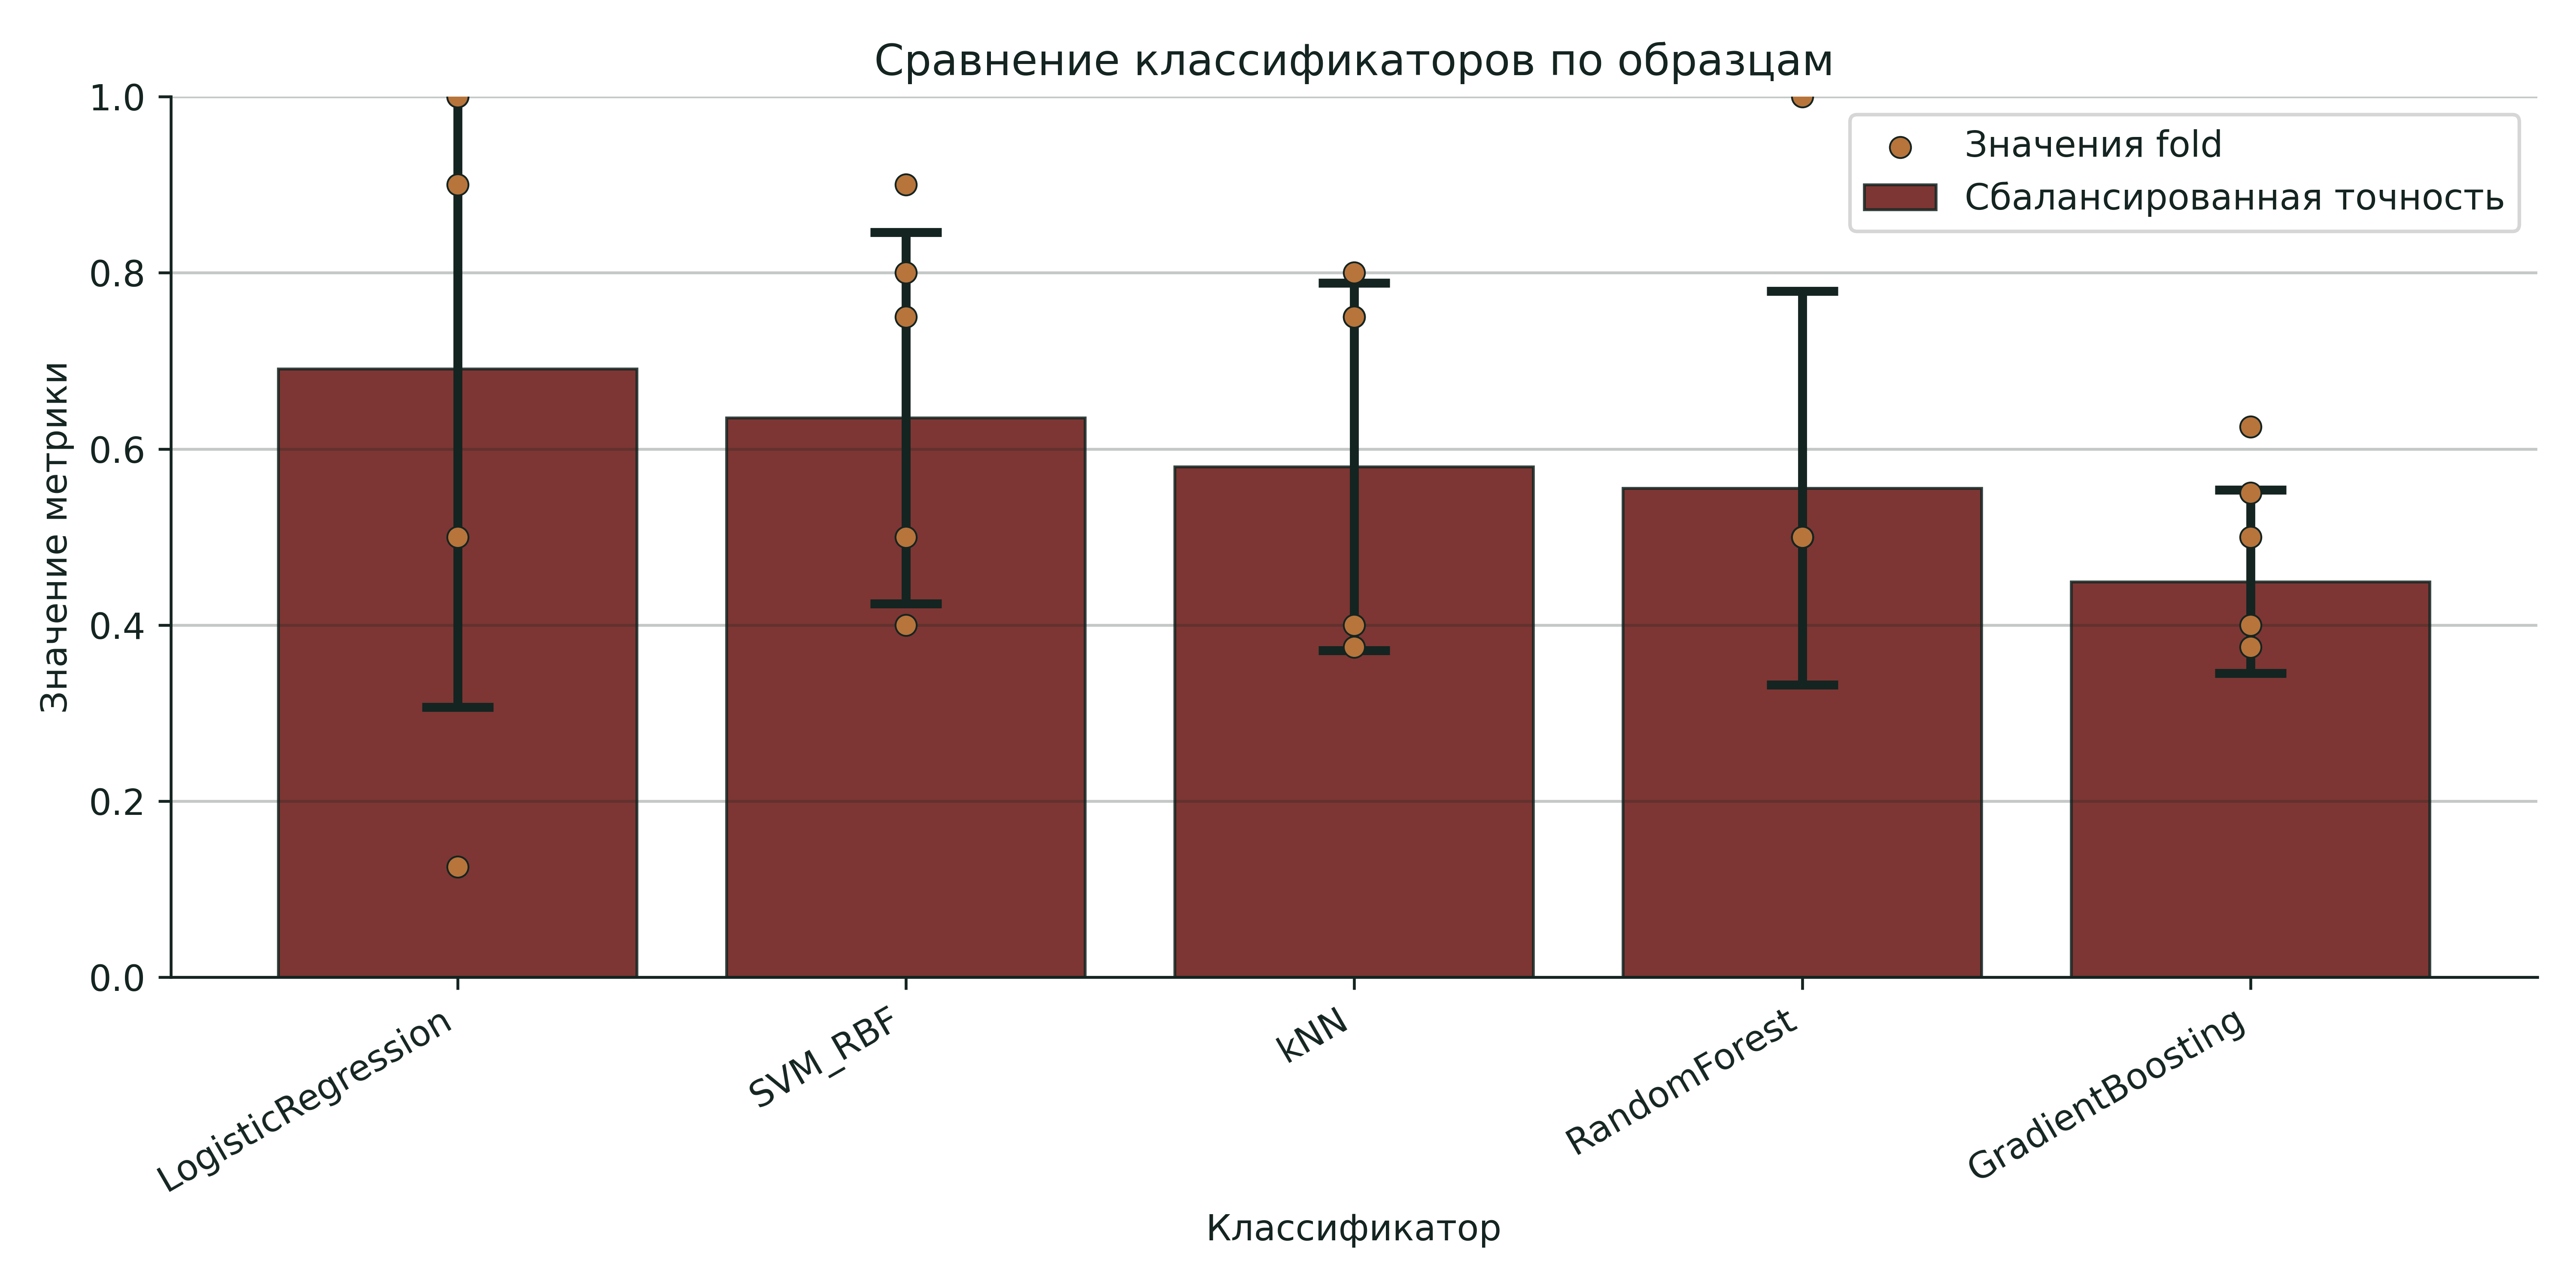
\includegraphics[width=0.9\textwidth]{figures/model_comparison.png}
    \caption{Сравнение классификаторов при обнаружении непровара по спектральным признакам}
    \label{fig:spectrum_model_comparison}
\end{figure}

Наилучший результат в базовой постановке был получен с использованием модели LogisticRegression. Для неё доля правильных ответов составила 0,750, сбалансированная точность --- 0,691, полнота для класса непровара --- 0,556, а F1-мера для класса непровара --- 0,556.

Формально доля правильных ответов выглядит приемлемой, однако для данной задачи она не является достаточной характеристикой качества. В выборке преобладают образцы с полным проплавлением, поэтому модель может получать сравнительно высокое значение точности даже при недостаточно хорошем обнаружении непровара. В базовом режиме LogisticRegression обнаружила только 5 из 9 образцов с непроваром. Следовательно, такая модель не может рассматриваться как достаточно надёжный самостоятельный детектор дефекта.

\section{Чувствительный режим обнаружения непровара}

Для задачи контроля качества пропуск дефекта является более критичной ошибкой, чем ложное направление нормального образца на дополнительную проверку. Поэтому дополнительно был рассмотрен чувствительный режим классификации. Его идея состояла в изменении порога принятия решения для модели, выдающей вероятность или оценку принадлежности к классу непровара.

В стандартной бинарной классификации образец обычно относится к дефектному классу при вероятности выше 0,5. В данной работе порог был уменьшен, чтобы повысить чувствительность модели к непровару. При этом порог не подбирался таким образом, чтобы все образцы автоматически относились к дефектным. Такой вариант не имел бы практического смысла.

Наилучший чувствительный режим был получен для модели LogisticRegression при пороге 0,45. В этом случае доля правильных ответов составила 0,750, сбалансированная точность --- 0,725, точность для класса непровара --- 0,545, полнота для класса непровара --- 0,667, а F1-мера для класса непровара --- 0,600.

Матрица ошибок для данного режима приведена на рис.~\ref{fig:best_sensitive_confusion_matrix}. Из 9 образцов с непроваром модель обнаружила 6 и пропустила 3. При этом 5 образцов с полным проплавлением были ошибочно отнесены к дефектным.

\begin{figure}[H]
    \centering
    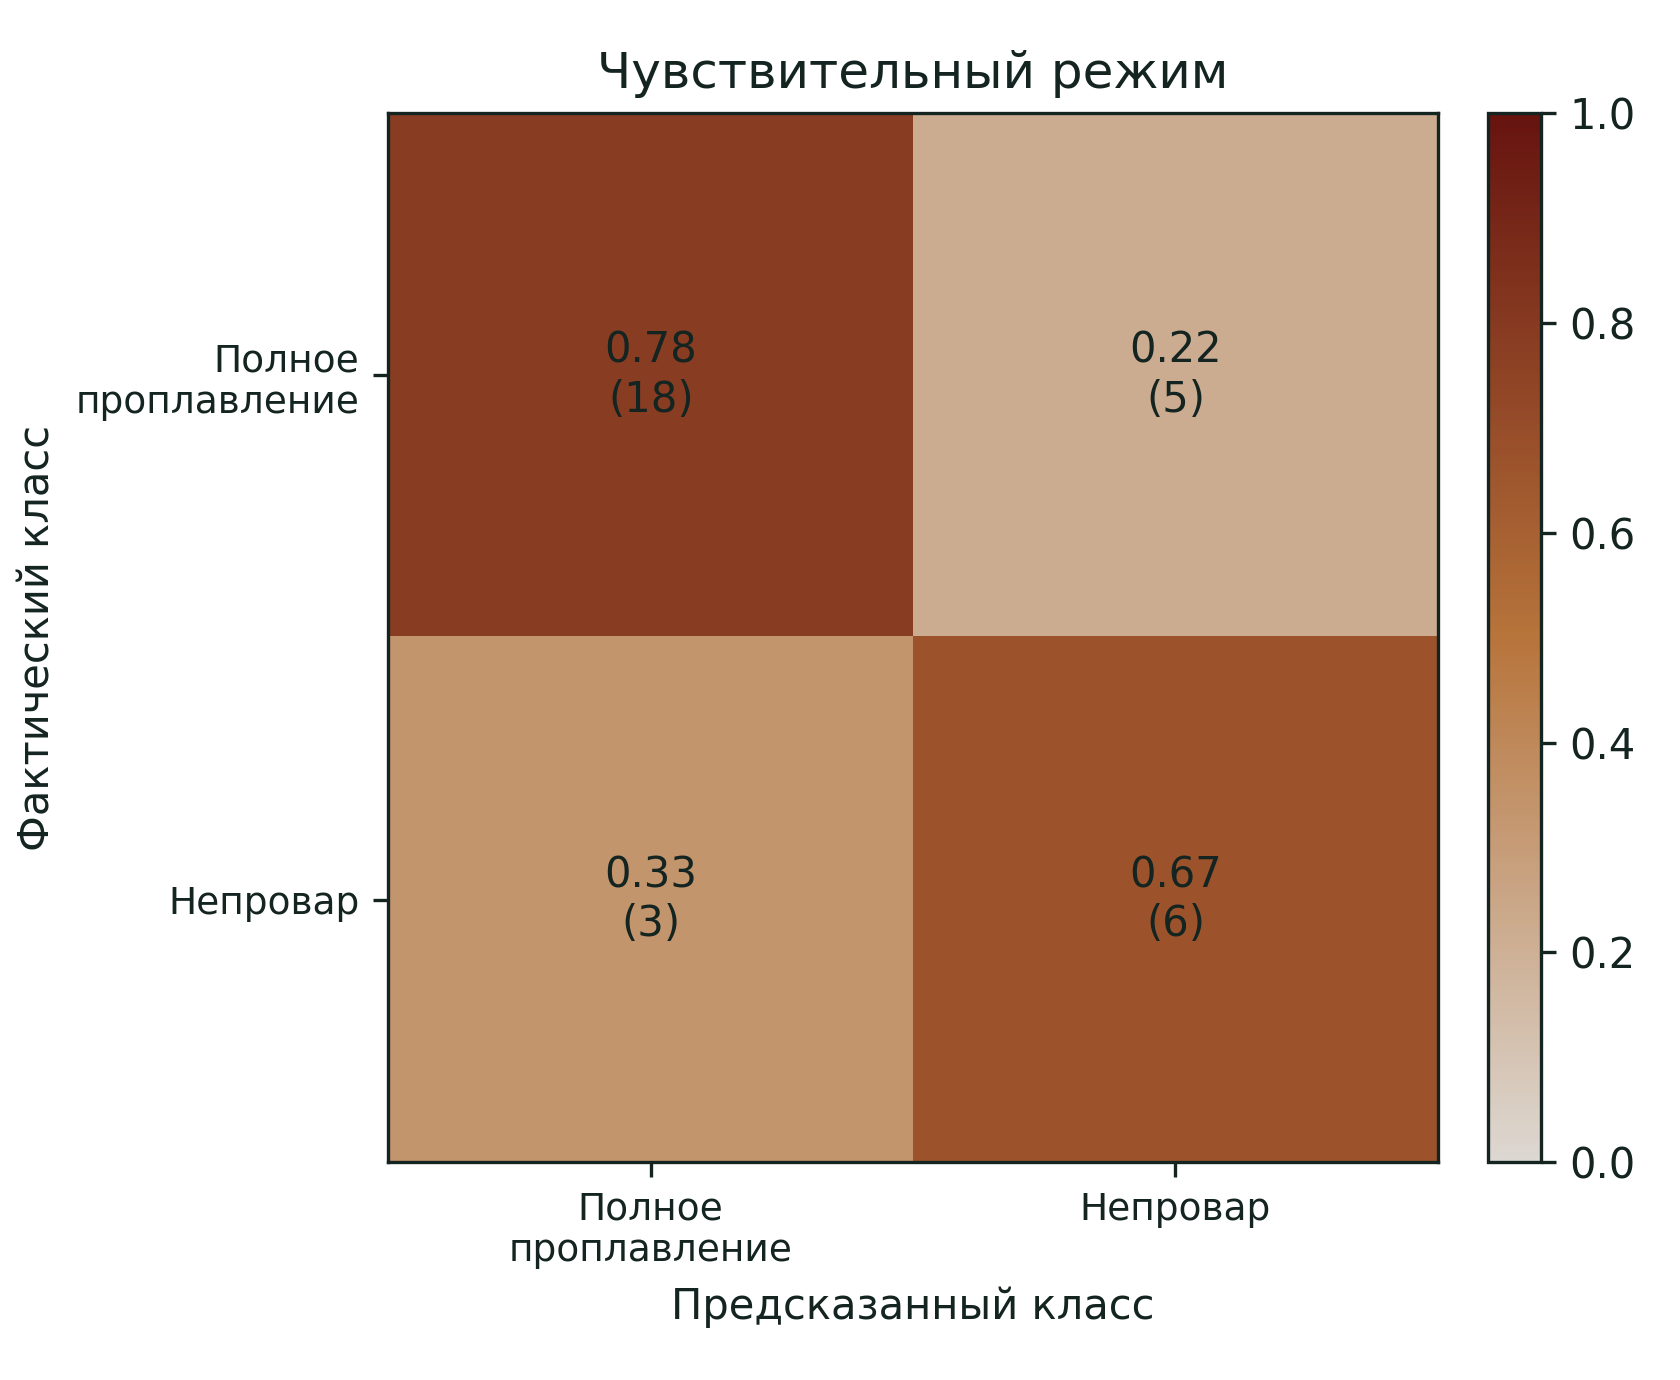
\includegraphics[width=0.72\textwidth]{figures/best_sensitive_confusion_matrix.png}
    \caption{Матрица ошибок для чувствительного режима LogisticRegression}
    \label{fig:best_sensitive_confusion_matrix}
\end{figure}

Таким образом, чувствительный режим не устраняет ошибки полностью, но меняет их структуру в более приемлемую для задачи контроля качества сторону. Модель чаще обнаруживает непровар, но ценой увеличения числа ложных срабатываний. С практической точки зрения такой результат можно рассматривать как вспомогательный индикатор: он не заменяет окончательный контроль качества, но может использоваться для выделения образцов, требующих дополнительной проверки.

\section{Сравнение чувствительных режимов разных моделей}

Для проверки того, что выбранный режим LogisticRegression не является случайным частным случаем, была выполнена аналогичная настройка чувствительности для разных моделей. Для каждой модели подбирался порог, обеспечивающий более высокую чувствительность к классу непровара при сохранении нетривиального поведения классификатора.

Результаты сравнения чувствительных режимов приведены на рис.~\ref{fig:sensitive_model_comparison}. На диаграмме модели сравниваются по полноте обнаружения непровара. Отдельные точки показывают значения этой метрики на отдельных разбиениях при кросс-валидации.

\begin{figure}[H]
    \centering
    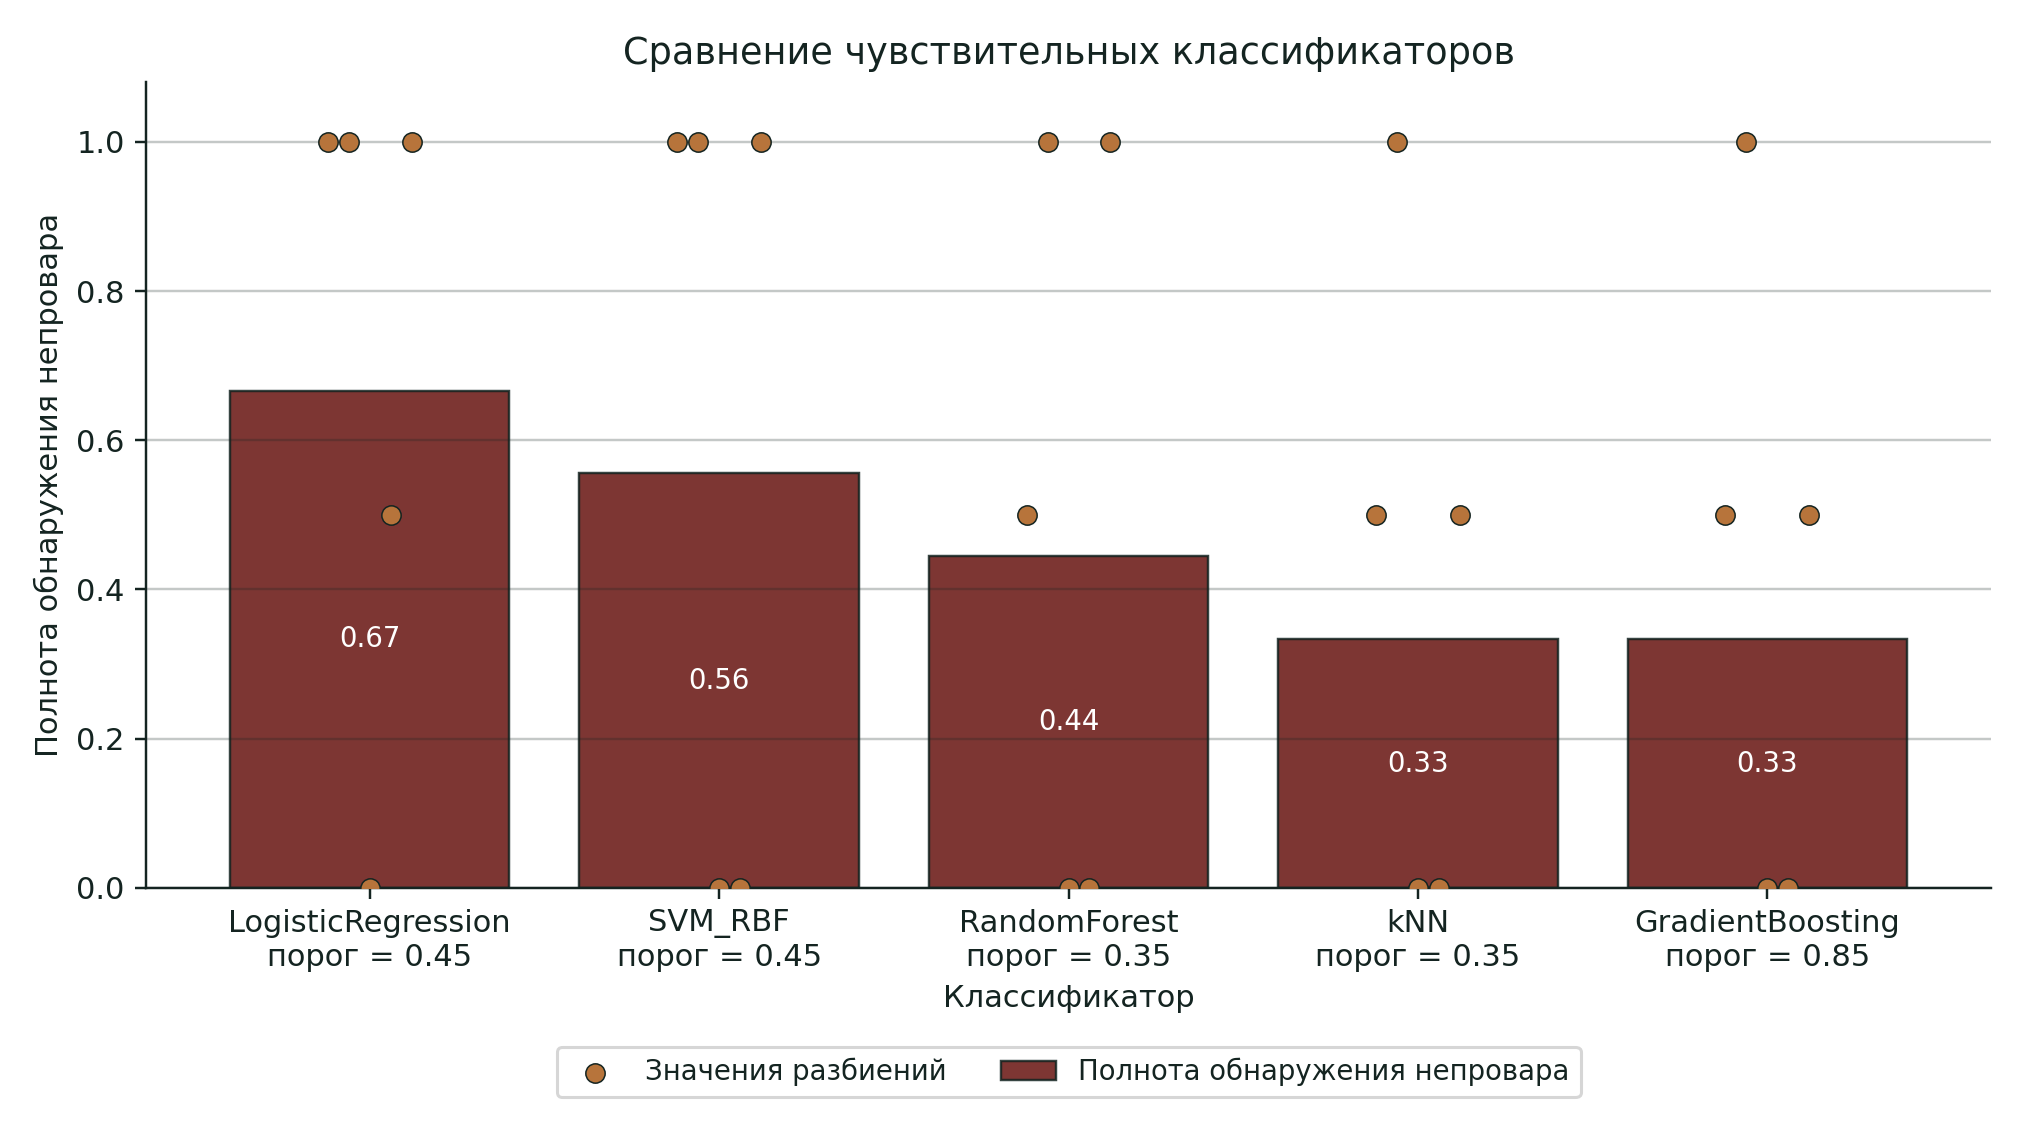
\includegraphics[width=0.9\textwidth]{figures/sensitive_model_comparison_top5.png}
    \caption{Сравнение чувствительных режимов классификации непровара}
    \label{fig:sensitive_model_comparison}
\end{figure}

Полученные результаты показывают, что повышение чувствительности к непровару возможно, но сопровождается ростом числа ложных срабатываний. Среди рассмотренных моделей наиболее приемлемый компромисс был получен для LogisticRegression. Эта модель не дала максимального формального улучшения по всем метрикам, однако обеспечила более понятное и устойчивое поведение при малом числе образцов.

\section{Дополнительные проверки постановки задачи}

Также была проверена схема голосования по спектрам. В этом варианте сначала классифицировались отдельные спектры, после чего для каждого образца вычислялась доля спектров, отнесённых к непровару. Образец считался дефектным, если эта доля превышала заданный порог. Лучший вариант был получен для SVM-RBF при условии, что доля спектров, отнесённых к непровару, составляет не менее 0,7. При этом доля правильных ответов составила 0,781, сбалансированная точность --- 0,713, полнота для класса непровара --- 0,556, а F1-мера для класса непровара --- 0,588.

Несмотря на более высокую долю правильных ответов, схема голосования не улучшила обнаружение непровара по сравнению с чувствительным режимом LogisticRegression. Поэтому она рассматривалась только как дополнительная проверка, а не как основная постановка анализа.

\section{Анализ информативности признаков}

Для интерпретации полученной модели был выполнен анализ информативности признаков LogisticRegression. Результат приведён на рис.~\ref{fig:feature_importance_logreg}. Следует учитывать, что при малом числе образцов интерпретация отдельных коэффициентов должна рассматриваться осторожно. Тем не менее такой анализ позволяет понять, какие группы признаков чаще участвуют в принятии решения.

\begin{figure}[H]
    \centering
    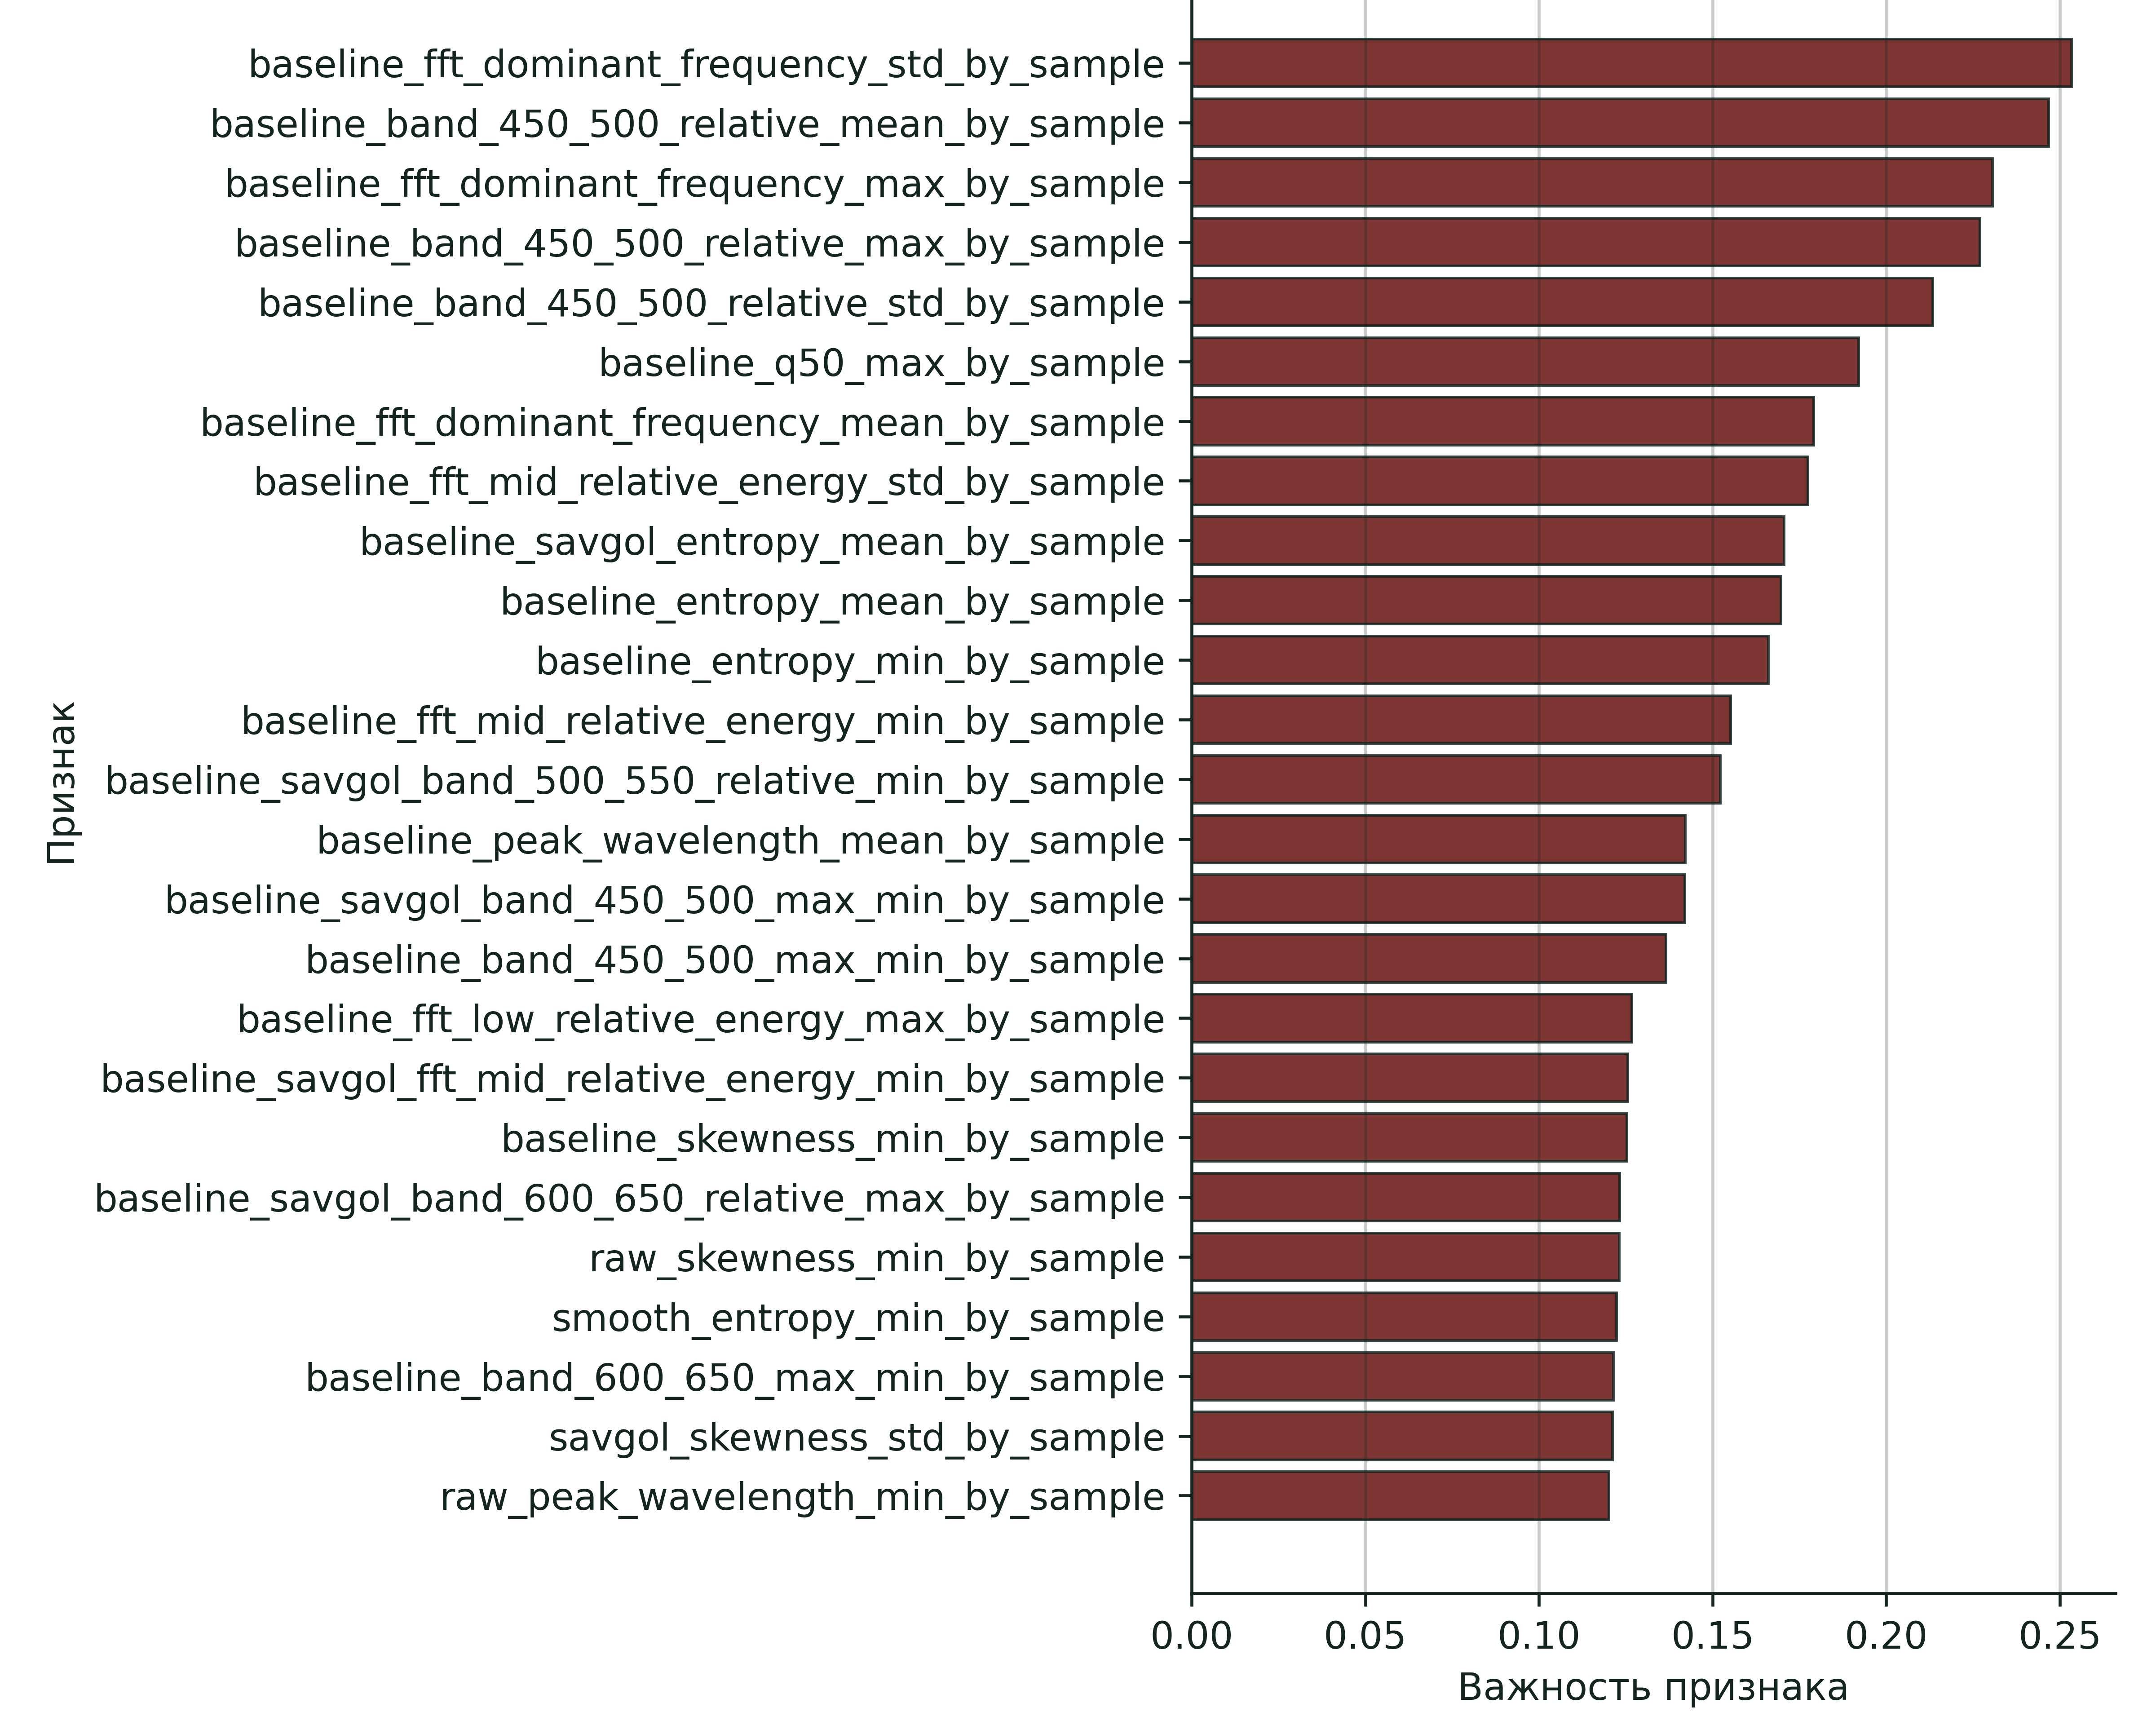
\includegraphics[width=0.9\textwidth]{figures/feature_importance_LogisticRegression.png}
    \caption{Информативность признаков для модели LogisticRegression}
    \label{fig:feature_importance_logreg}
\end{figure}

Среди значимых признаков присутствовали характеристики общего уровня интенсивности, формы спектрального распределения, диапазонные признаки, а также признаки, рассчитанные после предварительной обработки спектра. Это указывает на то, что модель использует не один отдельный параметр, а совокупность характеристик спектрального сигнала. Такой результат согласуется с общей логикой анализа оптических данных: для диагностики качества сварки обычно недостаточно одного простого признака, поэтому требуется многомерное описание сигнала.

В то же время нельзя утверждать, что отдельные признаки имеют универсальную физическую интерпретацию. Их значимость получена на ограниченной экспериментальной выборке и зависит от выбранной схемы обработки, состава образцов и особенностей расположения спектрометрической системы.

\section{Обсуждение ограничений спектрометрического подхода}

Полученные результаты требуют осторожной интерпретации. В отличие от фотодиодной системы, где временное окно может рассматриваться как локальный фрагмент процесса, в спектрометрической части работы ситуация сложнее. Спектрометр был закреплён статично относительно стола и регистрировал излучение из фиксированной области пространства. Поэтому последовательность спектров не является прямым аналогом локального контроля вдоль всего сварного шва.

Второе ограничение связано с разметкой. Величина \(h_i\) была определена по результатам макроанализа и относится к образцу, а не к отдельному спектру. При этом отсутствует информация, позволяющая однозначно сопоставить конкретный спектр с конкретным макрошлифом. Поэтому классификация отдельных спектров не является физически полностью корректной, а переход к агрегации признаков на уровне образца является более обоснованным.

Третье ограничение связано с объёмом выборки. В основной постановке рассматривались 32 образца, из которых только 9 соответствовали непровару. При таком количестве дефектных образцов качество моделей существенно зависит от состава разбиений кросс-валидации. Это ограничивает возможность делать жёсткие выводы о надёжности классификатора.

Наконец, слабый непровар может слабо отличаться по спектральному отклику от полного проплавления. Поэтому даже при использовании сглаживания, коррекции базовой линии и многомерного набора признаков разделение классов остаётся неполным. Наиболее удачный чувствительный режим позволил обнаружить 6 из 9 образцов с непроваром, однако 3 дефектных образца всё равно были пропущены.

Таким образом, спектрометрические признаки в текущей постановке содержат некоторую информацию, связанную с качеством сварного соединения, но не обеспечивают устойчивого самостоятельного детектора непровара. Более корректно рассматривать спектрометрический канал как дополнительный диагностический источник. Для повышения качества требуется либо большее число размеченных дефектных образцов, либо локальная разметка спектров, либо объединение спектральных признаков с сигналами других датчиков.

\chapterconclusion

Была рассмотрена возможность оценки качества сварного соединения по сигналам спектрометрической системы. В отличие от анализа фотодиодных данных, объектом первичного анализа являлся не временной фрагмент сигнала, а спектральное распределение интенсивности излучения по длинам волн. Для анализа был выбран основной спектрометрический канал \texttt{1712307U3} с диапазоном длин волн \(467,396\)--\(708,946\)~нм.

Для спектральных данных была построена последовательность обработки, включающая чтение Raw8-файлов, сопоставление спектров с результатами макроанализа, предварительный отбор информативных спектров, сглаживание, коррекцию базовой линии и извлечение признаков. Поскольку величина \(h_i\) задана на уровне образца, основной объект классификации был выбран в виде образца, а признаки отдельных спектров агрегировались по идентификатору образца.

Качественная оценка была сформулирована как бинарная классификация по условию \(h_i = 0\) или \(h_i > 0\). Базовая модель LogisticRegression показала accuracy 0,750 и balanced accuracy 0,691, однако обнаружила только 5 из 9 образцов с непроваром. Поэтому дополнительно был рассмотрен чувствительный режим классификации. При пороге 0,45 модель LogisticRegression обнаружила 6 из 9 образцов с непроваром, но при этом ошибочно отнесла 5 образцов с полным проплавлением к дефектным.

Проверка альтернативных постановок показала, что классификация отдельных спектров практически не обеспечивает устойчивого разделения классов. Схема голосования по спектрам несколько повышала accuracy, но не улучшала обнаружение непровара относительно чувствительного режима. Это подтверждает, что для имеющейся разметки более корректной является классификация на уровне образца.

Таким образом, спектрометрическая система в рассматриваемой постановке может использоваться как дополнительный источник диагностической информации, но не даёт достаточно надёжного самостоятельного классификатора непровара. Для дальнейшего повышения качества необходимы расширение набора дефектных образцов, локальная разметка спектров относительно положения дефекта или совместное использование спектральных признаков с сигналами фотодиодной системы.